% Report-style version of paper_draft/main.tex (same evidence, same numbers; shorter and less formal).
% Numbers are those checked in paper_draft/claim_evidence.csv. Compile: latexmk -pdf report.tex
\documentclass[11pt,a4paper]{article}
\usepackage[T1]{fontenc}
\usepackage[utf8]{inputenc}
\usepackage{lmodern}
\usepackage[margin=2.3cm]{geometry}
\usepackage{amsmath}
\usepackage{graphicx}
\usepackage{booktabs,tabularx}
\usepackage{xcolor}
\usepackage[skins]{tcolorbox}
\usepackage{enumitem}
\usepackage{parskip}
\usepackage[round,authoryear]{natbib}
\usepackage{microtype}
\usepackage[font=small,labelfont=bf]{caption}
\usepackage{fancyhdr}
\usepackage[colorlinks=true,linkcolor=blue!50!black,citecolor=blue!50!black,urlcolor=blue!50!black]{hyperref}
\usepackage[capitalise,noabbrev]{cleveref}
\graphicspath{{../figures/}}
\setlist{itemsep=2pt,topsep=3pt}
\pagestyle{fancy}\fancyhf{}
\fancyfoot[L]{\footnotesize XRB-pilot summary report}
\fancyfoot[R]{\footnotesize\thepage}
\renewcommand{\headrulewidth}{0pt}
\newcommand{\ci}[2]{$[#1,\,#2]$}

\begin{document}

\begin{center}
{\LARGE\bfseries Black holes vs neutron stars from X-ray colours\\[3pt] and low-frequency variability}\\[8pt]
{\large XRB-pilot summary report (analysis rounds v1--v13)}\\[4pt]
{\small October 2026 \quad$\cdot$\quad repository \texttt{Chipwwwwww/XRB-pilot}, commit \texttt{666c2e0}}
\end{center}

\begin{tcolorbox}[colback=blue!3,colframe=blue!40!black,boxrule=0.6pt,arc=2pt,title=Key findings,fonttitle=\bfseries]
\begin{enumerate}[leftmargin=1.4em]
\item \textbf{Two X-ray colours do the spectral work.} On 31 RXTE sources that were each left out of training in turn,
a logistic regression on two hardness ratios separated BHs from NSs with a source-level AUC of 0.923
\ci{0.804}{0.994}. The full spectrum, extra energy bands, 17 times more observations and a search over eight
algorithms did not improve on this.
\item \textbf{Colours work in soft states and struggle in hard states.} The observation-level AUC was 0.954 in
soft-like observations and 0.646 in hard-like ones. The same pattern holds in every NICER set.
\item \textbf{Low-frequency variability (0.016--4~Hz) fills much of the hard-state gap.} Adding three rms amplitudes to
the colours raised the hard-like AUC by +0.264 in RXTE, and by +0.17 to +0.25 with a random forest in every NICER set.
\item \textbf{The gain held up in a final test fixed in advance.} The test used 198 NICER observations not used before,
background-corrected with the 3C50 model, with every processing and modelling choice frozen before the data were
downloaded. The hard-like AUC rose from 0.680 to 0.864 ($+0.184$ \ci{+0.049}{+0.337}).
\item \textbf{Next step: new black holes.} All new data so far are new observations of sources already in the sample;
the decisive test is on BHs never used before.
\end{enumerate}
\end{tcolorbox}

\section{What we asked}
Dynamical masses and type-I bursts or pulsations are the only secure ways to tell a BH from an NS in an X-ray binary.
Many sources, especially new transients, have neither, so the X-ray data themselves are used. Published
machine-learning classifiers on RXTE and MAXI data report 87--94\% accuracies
\citep{Pattnaik2021,deBeurs2022,Garg2026}. Such headline numbers leave open what the classifier is actually using and
where it fails. We asked four things, always testing on sources the model had not seen:
\begin{enumerate}[leftmargin=1.4em]
\item How much of the spectral information is captured by two X-ray colours?
\item How does performance depend on accretion state?
\item In hard states, where colours overlap, does low-frequency variability add information?
\item Does that gain survive a second instrument, background correction, and new observations analysed with a frozen
pipeline?
\end{enumerate}

\section{Data and approach}

\paragraph{Sources.}
BHs are dynamically confirmed systems \citep{CorralSantana2016,Marcel2026}. NSs are type-I bursters
\citep{Galloway2008,Galloway2020} plus a few pulsars. Across both instruments there are 86 sources, 16 of them BHs.

\paragraph{Samples.}
\Cref{tab:samples} lists the samples:
\begin{itemize}[leftmargin=1.4em]
\item an RXTE development sample of 31 sources and 456 observations;
\item 26 external RXTE sources;
\item three non-overlapping sets of NICER observations of one source list (N1, N2, N3), plus a re-analysis of N1+N2
with the 3C50 background model \citep{Remillard2022}.
\end{itemize}

\begin{table}[h]
\centering\small
\caption{Samples. Hard-like observations with BH/NS source counts in brackets.}\label{tab:samples}
\setlength{\tabcolsep}{4.5pt}
\begin{tabular}{@{}l l r r r l l@{}}
\toprule
Sample & Instrument & Obs. & Sources (BH/NS) & Hard-like obs & Background & How tested \\
\midrule
Development & RXTE/PCA & 456 & 31 (7/24) & 180 (7/17) & \textsc{pcabackest} & source left out \\
External & RXTE/PCA & 379 & 26 (7/19) & 99 (5/15) & \textsc{pcabackest} & frozen models \\
N1 & NICER/XTI & 366 & 63 (9/54) & 144 (7/32) & none & source left out \\
N2 (new obs.) & NICER/XTI & 318 & 60 (9/51) & 143 (9/33) & none & frozen models \\
N1+N2 & NICER/XTI & 534 & 58 (9/49) & 202 (8/34) & 3C50 & source left out \\
N3 (new obs.) & NICER/XTI & 198 & 35 (8/27) & 74 (8/19) & 3C50 & all frozen \\
\bottomrule
\end{tabular}
\end{table}

\paragraph{Features.}
\begin{itemize}[leftmargin=1.4em]
\item \textbf{H} (colours): two hardness ratios. For RXTE these are 7--10/5--7~keV and 16--25/10--16~keV; for NICER,
4--6/2--4~keV and 6--10/4--6~keV.
\item \textbf{T} (timing): fractional rms in 0.016--0.094, 0.10--1.0 and 1.0--4.0~Hz ($T_1$, $T_2$, $T_3$). It is
measured from cross-spectra between detector units, which removes the Poisson noise level.
\end{itemize}

\paragraph{State classes.}
Total rms in 0.1--4~Hz (RXTE) or 0.1--10~Hz (NICER) above 0.10 is ``hard-like''; below 0.075 is ``soft-like''. The
thresholds come from \citet{RemillardMcClintock2006}.

\paragraph{Models and evaluation.}
\begin{itemize}[leftmargin=1.4em]
\item Logistic regression (LR) and random forest (RF), with fixed settings.
\item Models are always trained without the source being tested.
\item For the new NICER observations (N2, N3), each source is scored by a model trained on the earlier data with that
source removed.
\item Main metric: AUC, computed per observation and per source (a source's score is the mean of its observations).
\item Intervals: 95\% source-level bootstrap (2000 draws).
\end{itemize}

\section{Results}

\subsection{Two colours carry the spectral information}
On the RXTE development sample, the two-colour LR reached:
\begin{itemize}[leftmargin=1.4em]
\item a source-level AUC of 0.923 \ci{0.804}{0.994};
\item 26 of 31 sources correctly classified (5 of 7 BHs, 21 of 24 NSs).
\end{itemize}
The misclassified sources were the BHs GRS~1915$+$105 and XTE~J1118$+$480 and the NSs HETE~J1900.1$-$2455,
KS~1731$-$260 and SAX~J1808.4$-$3658. With RF the source-level AUC was 0.905.

Giving the models more spectral information did not help (\cref{fig:colour}). The changes in source-level AUC were:
\begin{itemize}[leftmargin=1.4em]
\item adding the full 45-bin 5--25~keV shape: $-0.048$ (LR), $-0.012$ (RF);
\item extending to 3--25~keV: $-0.018$ (LR), $-0.054$ (RF);
\item adding 25--60~keV HEXTE colours: $-0.048$ (LR), $0.000$ (RF);
\item training on all 7949 available observations instead of 456: $0.000$;
\item a nested search over eight algorithms: $-0.173$ relative to the two-colour LR.
\end{itemize}

Leaving whole sources out matters. Splitting the same data by observation instead raised balanced accuracy by 0.04--0.16,
because the model then partly recognises sources it has already seen.

\begin{figure}[h]
\centering
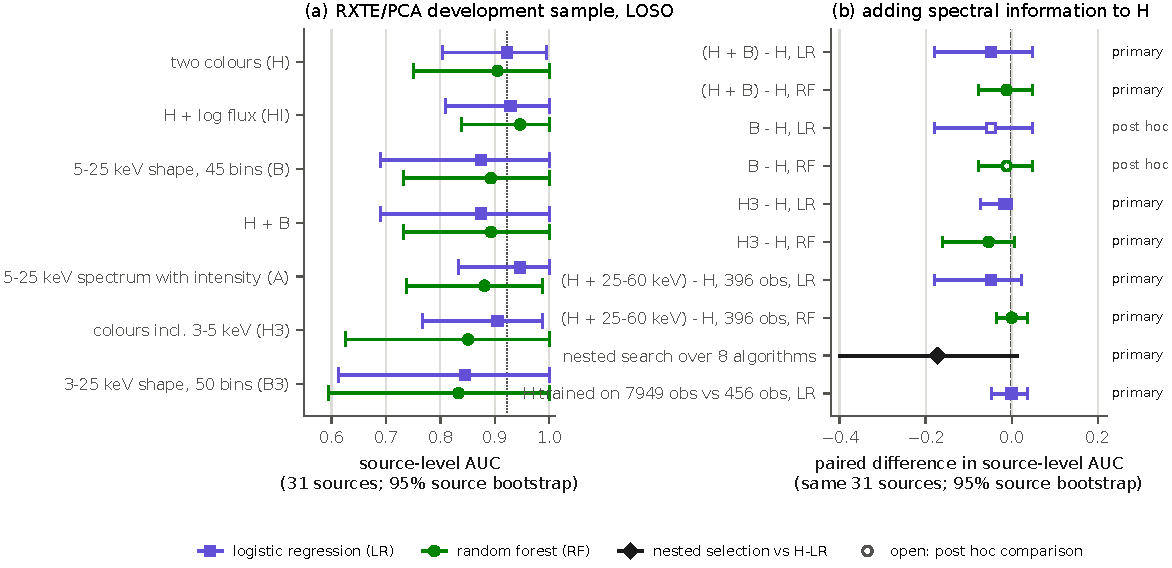
\includegraphics[width=\textwidth]{fig2_colour_ablation.pdf}
\caption{RXTE development sample (31 sources). (a) Source-level AUC of each spectral representation. (b) Change in
source-level AUC when spectral information is added to the two colours. Bars: 95\% source bootstrap.}\label{fig:colour}
\end{figure}

\subsection{The difficulty is the hard state}
Split by state, the colour--colour diagrams show a clear picture (\cref{fig:states}a--d). In soft-like observations, BHs
and NSs sit in different places. In hard-like observations they overlap. The colour-only LR on RXTE had an
observation-level AUC of:
\begin{itemize}[leftmargin=1.4em]
\item \textbf{0.954} in soft-like observations;
\item \textbf{0.646} in hard-like observations;
\item a difference of +0.309 \ci{+0.099}{+0.510}.
\end{itemize}
NICER shows the same split. Colour-only hard-like AUCs were 0.50--0.68 with LR and 0.67--0.75 with RF, against
0.83--0.95 in soft-like observations (\cref{fig:states}e). All seven RXTE BHs have hard-like observations, so this is
the case that every BH presents at some point in an outburst.

\begin{figure}[h]
\centering
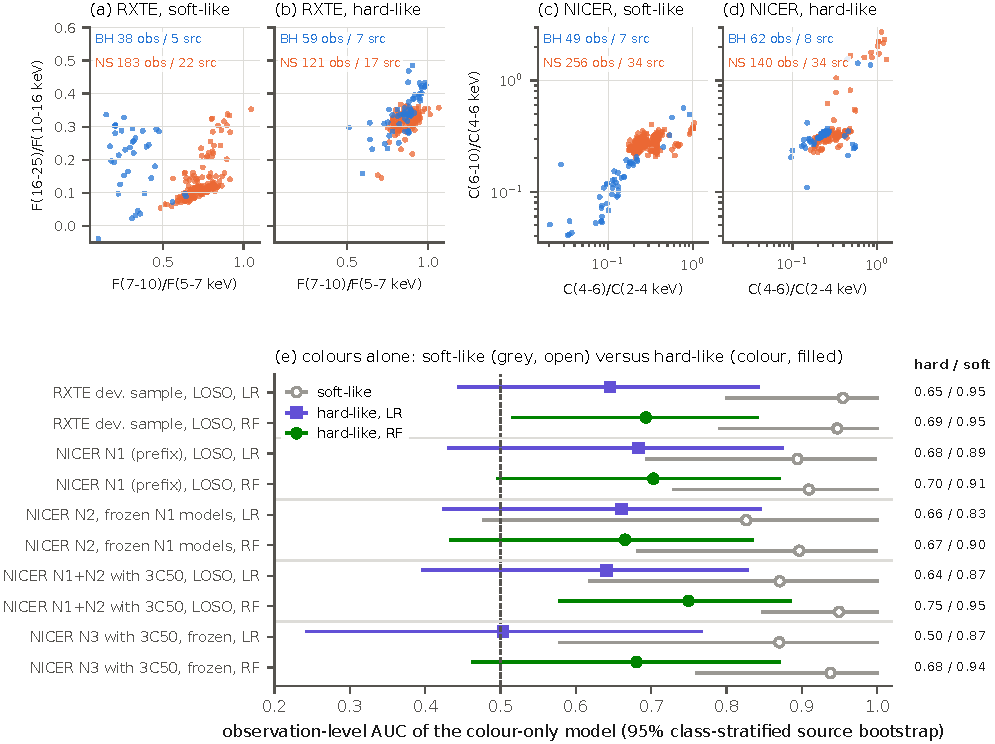
\includegraphics[width=\textwidth]{fig3_states.pdf}
\caption{(a--d) Colour--colour diagrams for soft-like and hard-like observations (RXTE development sample; NICER N1+N2
after 3C50 correction). (e) Colour-only AUC in soft-like (grey) and hard-like (colour) observations for each sample.}\label{fig:states}
\end{figure}

\subsection{Low-frequency variability adds hard-state information}
Adding $T_1$--$T_3$ to the colours improved hard-like classification in every sample (\cref{fig:gain}).
\begin{itemize}[leftmargin=1.4em]
\item \textbf{RXTE development sample.} The LR hard-like AUC rose from 0.646 to 0.910, a gain of $+0.264$
\ci{+0.048}{+0.455}. With RF the gain was $+0.230$ \ci{+0.074}{+0.408}. Per source, the AUC rose from 0.748 to 0.933.
\item \textbf{RXTE external sources.} The colours alone already gave 0.817, and the gain was smaller: $+0.064$
\ci{-0.185}{+0.367}.
\item \textbf{NICER N1.} The gain was $+0.112$ \ci{-0.004}{+0.229} with LR and $+0.236$ \ci{+0.104}{+0.372} with RF.
Full event files gave $+0.107$ (LR) and $+0.219$ (RF).
\item \textbf{RXTE and NICER pooled.} The gain was $+0.145$ \ci{+0.028}{+0.257}.
\end{itemize}

In soft-like observations, the colours already separate the classes and timing added essentially nothing ($+0.036$ in
RXTE). The variability information is therefore specific to the hard state.

The band that matters differs between instruments. In RXTE the lowest band ($T_1$) helped most: hard-like AUC 0.926
with $T_1$ alone, 0.874 with $T_2$, 0.654 with $T_3$. In NICER, $T_2$ ($+0.143$) and $T_3$ ($+0.115$) helped more than
$T_1$ ($+0.048$). The two instruments also cover different energies: all PCA channels for RXTE, 2--10~keV for NICER.

RF gains were consistently larger and more stable than LR gains: +0.17 to +0.25, against +0.07 to +0.26. This
suggests that the relation between colours, variability and source type is not linear.

\begin{figure}[h]
\centering
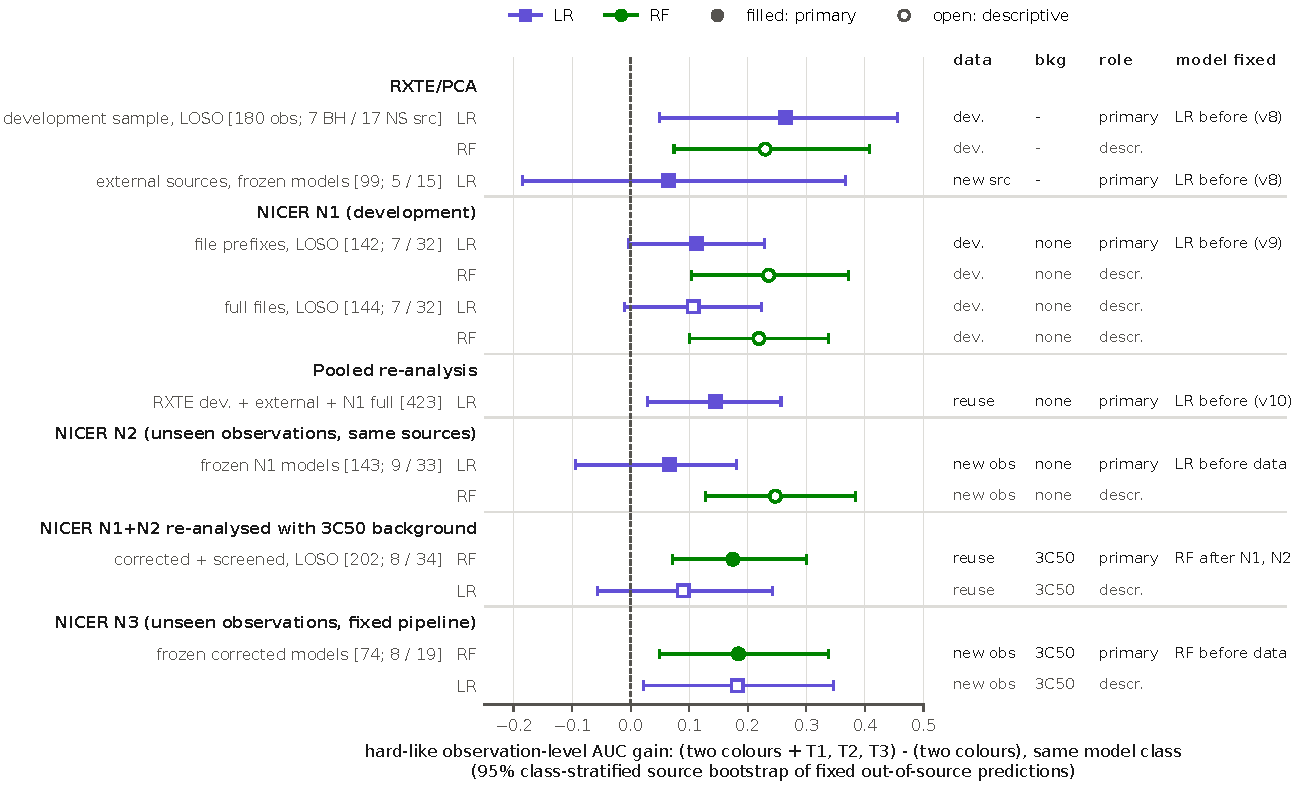
\includegraphics[width=\textwidth]{fig4_timing_gain.pdf}
\caption{Hard-like AUC gain from adding $T_1$--$T_3$ to the two colours, for every sample (violet: LR; green: RF). The
right-hand columns give the data status, background treatment, whether the comparison was the main test of its round,
and when the model was fixed. Bars: 95\% source bootstrap.}\label{fig:gain}
\end{figure}

\subsection{Background correction and new observations}
Two further steps tested whether the gain is real or an artefact of how the NICER data were handled.

\paragraph{N2: new observations, models frozen.}
On 318 NICER observations never used before, the frozen N1 models gave:
\begin{itemize}[leftmargin=1.4em]
\item RF: hard-like gain $+0.247$ \ci{+0.128}{+0.384} (0.665 to 0.912);
\item LR: $+0.066$ \ci{-0.095}{+0.180}, with its decision threshold transferring poorly to the new data.
\end{itemize}

\paragraph{3C50 background correction (N1+N2).}
The median background fraction was below 1\%. After correction, the RF gain was $+0.174$ \ci{+0.071}{+0.300}, from
0.750 to 0.924. The background is therefore not what drives the gain. From this point on, RF was the main model.

\paragraph{N3: everything fixed in advance.}
For a third set of observations, the 3C50 pipeline, state thresholds, features and RF models were all frozen before any
data were downloaded. Of 238 accepted observations, 198 passed the background screening. The results are in
\cref{tab:v13} and \cref{fig:v13}:
\begin{itemize}[leftmargin=1.4em]
\item the hard-like AUC rose from 0.680 to \textbf{0.864}, a gain of \textbf{$+0.184$ \ci{+0.049}{+0.337}};
\item LR showed a similar gain ($+0.182$);
\item removing any single BH left gains between $+0.146$ and $+0.212$;
\item computing the timing features only within the background model's good-time intervals gave $+0.190$;
\item in soft-like observations the gain was zero ($+0.005$);
\item per source, the AUC rose from 0.717 to 0.842 ($+0.125$ \ci{-0.053}{+0.303}). This is the same direction, but
27 sources are too few to pin it down.
\end{itemize}

\begin{table}[h]
\centering\small
\caption{N3: new NICER observations, frozen pipeline and models. 95\% source-bootstrap intervals.}\label{tab:v13}
\begin{tabular}{@{}l l l l@{}}
\toprule
Hard-like metric & Colours only & Colours + timing & Gain \\
\midrule
Observation AUC, RF (74 obs) & 0.680 & 0.864 & $+0.184$ \ci{+0.049}{+0.337} \\
Observation AUC, LR & 0.503 & 0.685 & $+0.182$ \ci{+0.022}{+0.347} \\
Observation balanced accuracy, RF & 0.607 & 0.744 & $+0.137$ \ci{+0.019}{+0.275} \\
Source AUC, RF (27 sources) & 0.717 & 0.842 & $+0.125$ \ci{-0.053}{+0.303} \\
Soft-like observation AUC, RF & 0.938 & 0.943 & $+0.005$ \ci{-0.015}{+0.035} \\
\bottomrule
\end{tabular}
\end{table}

\begin{figure}[h]
\centering
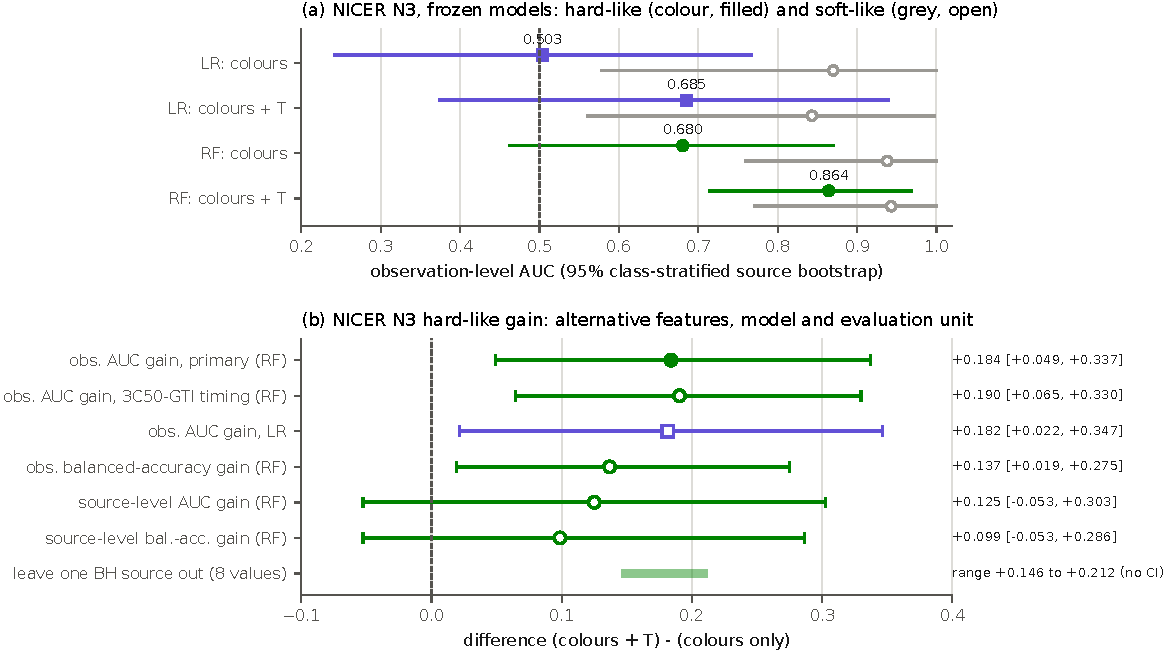
\includegraphics[width=0.9\textwidth]{fig5_v13.pdf}
\caption{N3. (a) AUC of the four frozen models in hard-like (colour) and soft-like (grey) observations. (b) The hard-like
gain under alternative features, model and evaluation unit, and with one BH left out at a time.}\label{fig:v13}
\end{figure}

\subsection{Side result: BHs vary more slowly at the same colour}
We also compared a characteristic variability frequency $\nu_c$ between BHs and NSs with matched colours. BHs came out
lower in every NICER set, by 0.3--0.7~dex, which is a factor of about 2--5 (\cref{fig:nuc}). The pooled RXTE+NICER test
gave $p = 0.0012$, but individual sets ranged from $p = 0.02$ to $0.21$. The size of the difference also shrank when
possibly background-dominated observations were removed. This is an interesting lead; on its own it is not yet a result.

\begin{figure}[h]
\centering
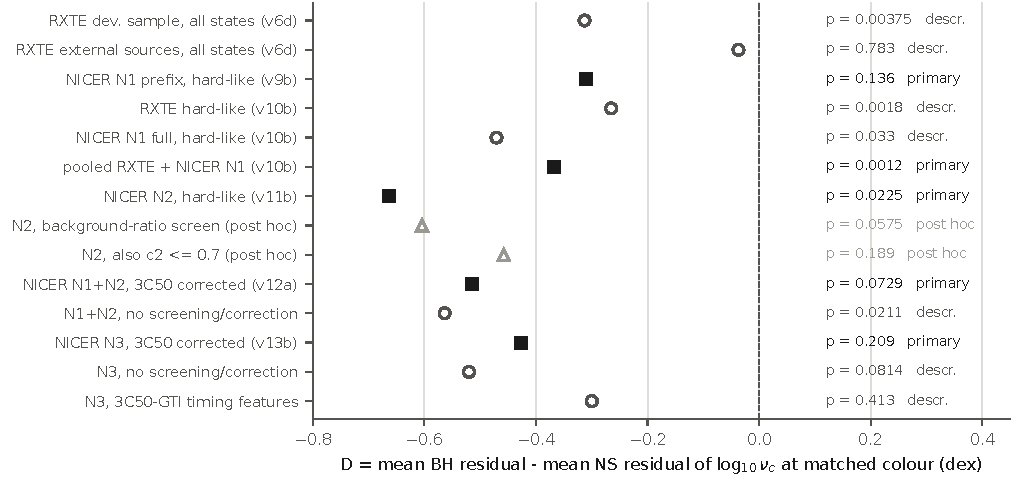
\includegraphics[width=0.85\textwidth]{figA1_nuc.pdf}
\caption{BH minus NS difference in $\log_{10}\nu_c$ at matched colour, for each sample and processing variant, with
permutation $p$-values. Squares mark the main test of each round.}\label{fig:nuc}
\end{figure}

\section{How this fits with earlier work}
\begin{itemize}[leftmargin=1.4em]
\item \textbf{Classifiers.} \citet{Pattnaik2021} classified RXTE spectra with a random forest and left whole sources out
of testing. They also noted that hard and intermediate states are the difficult cases. \citet{deBeurs2022} did the
same with MAXI colour--colour--intensity diagrams.
\item \textbf{What this work adds} is the breakdown of where the classifier's information comes from: two colours for
the spectrum, soft states for the colours, and low-frequency variability for the hard states.
\item \textbf{Observation-wise splits.} \citet{Garg2026} reached 90--94\% with neural networks on RXTE spectra, splitting
by observation. In our data that kind of split inflates accuracy by 0.04--0.16, so the two numbers measure different
things.
\item \textbf{Timing.} Timing as a BH/NS discriminant goes back to the high-frequency criterion of
\citet{SunyaevRevnivtsev2000}. Power-colour studies showed that BH and NS broad-band variability follow similar tracks
\citep{Heil2015,GardenierUttley2018}. Our result is that, at a given colour, the low-frequency amplitudes still carry
class information.
\end{itemize}

\section{Open items and next steps}
\begin{enumerate}[leftmargin=1.4em]
\item \textbf{Test on new BHs.} N2 and N3 are new observations of known sources, and only 16 confirmed BHs had usable
timing data. Applying the frozen N3 pipeline and RF to BHs and NSs never used here (for example new NICER transients)
is the most important next step.
\item \textbf{Total rms or band structure?} Hard-like is itself defined by total rms. Comparing colours + total rms
with colours + $T_1$--$T_3$ would show whether the gain comes from how much variability there is or from how it is
distributed in frequency.
\item \textbf{Weighting.} The observation-level AUC weights sources by their number of observations; for example
Cyg~X-1 has 7 of the 29 N3 BH observations. A per-source-weighted version and one that groups observations by outburst
would complete the picture.
\item \textbf{Physical controls.} Eddington ratio, inclination and NS type (atoll, Z source, millisecond pulsar) were
not controlled. They matter most for interpreting $\nu_c$.
\item \textbf{NICER background.} 3C50 could not process 2017--2018 data with the old gain calibration, which removed
about a quarter of the faint observations. Reprocessing those data would recover them.
\end{enumerate}

\appendix
\section{How the analysis developed}
\begin{center}\small
\begin{tabularx}{\textwidth}{@{}l >{\raggedright\arraybackslash}X >{\raggedright\arraybackslash}X@{}}
\toprule
Round & What was done & Main outcome \\
\midrule
v1--v3 & RXTE spectra, 31 sources; spectral representations; 3--25~keV & two colours match the full spectrum (AUC 0.92) \\
v4 & algorithm search, HEXTE, more observations, burst check & nothing beats two colours \\
v5--v6 & Standard-1 timing features; external sources & first sign of a timing gain \\
v7 & state classes; MINBAR bursts; MAXI & soft 0.954 vs hard 0.646 \\
v8 & timing within hard-like observations (RXTE) & hard-like gain +0.264 \\
v9--v10 & NICER N1; RXTE+NICER pooled & RF +0.236; pooled +0.145 \\
v11 & NICER N2, frozen models & RF +0.247; LR +0.066 \\
v12 & 3C50 background re-analysis & RF +0.174 \\
v13 & NICER N3, everything frozen before download & RF +0.184 [+0.049, +0.337] \\
\bottomrule
\end{tabularx}
\end{center}

Code, analysis plans, decision log and all result tables are in the repository. The full numbers behind this report
are checked in \texttt{paper\_draft/claim\_evidence.csv}. The long technical report is \texttt{report\_en/main.pdf}.

\bibliographystyle{plainnat}
\bibliography{references_report}

\end{document}
